% Created 2017-09-28 Jeu 14:17
\documentclass[11pt]{article}
\usepackage[margin=1.6in]{geometry}
\usepackage[T1]{fontenc}
%\usepackage{fixltx2e}
\usepackage{graphicx}
%\usepackage{longtable}
\usepackage{minted}
\usemintedstyle{colorful}
\setminted{fontsize=\footnotesize}
%\usepackage{wrapfig}
\usepackage{amsmath, amsthm}
%\usepackage{textcomp}
%\usepackage{marvosym}
%\usepackage{wasysym}
\usepackage{amssymb}
\usepackage{hyperref}
% Pour XeTeX
%\XeTeXdefaultencoding utf-8
\usepackage{fontspec}

\usepackage[style=alphabetic, backend=biber]{biblatex}
\addbibresource{Siphash.bib}
% Appel usuel à des packages
\usepackage{listings}
\usepackage[frenchb]{babel}
\lstset{
  %frame=tb,
  language=C,
  aboveskip=2mm,
  belowskip=2mm,
  showstringspaces=false,
  columns=flexible,
  basicstyle={\scriptsize\ttfamily},
  numbers=none,
  numberstyle=\footnotesize\color{gray},
  keywordstyle=\color{blue},
  commentstyle=\color{dkgreen},
  stringstyle=\color{mauve},
  breaklines=true,
  breakatwhitespace=true
  tabsize=3
}

\newenvironment{absolutelynopagebreak}
  {\par\nobreak\vfil\penalty0\vfilneg
   \vtop\bgroup}
  {\par\xdef\tpd{\the\prevdepth}\egroup
   \prevdepth=\tpd}

\usepackage{color}
\definecolor{dkgreen}{rgb}{0,0.6,0}
\definecolor{gray}{rgb}{0.5,0.5,0.5}
\definecolor{mauve}{rgb}{0.58,0,0.82}

\theoremstyle{definition}
\newtheorem*{mydef}{Définition}

\theoremstyle{definition}
\newtheorem*{myrem}{Remarque}

\theoremstyle{definition}
\newtheorem*{myex}{Exemple}

\theoremstyle{theorem}
\newtheorem*{myprop}{Proposition}

\theoremstyle{definition}
\newtheorem*{mydemo}{Démonstration}

\tolerance=1000
\setcounter{secnumdepth}{2}
\author{Borne, Duverney}
\date{}
\title{Siphash}

\begin{document}

\maketitle

\section{Transformation de l'entrée}
Afin de pouvoir implémenter l'algorithme \texttt{siphash} tel que décrit par ses auteurs,
nous devons transformer l'entrée, consistant en une séquence de mots de 8 bits, en une séquence de
mots sur 64 bits. Il est de plus demandé de stocker dans le dernier mot de 64 bits, la taille de l'entrée
modulo 256. Ayant eu des difficultés à interpréter certaines indications des auteurs (notation little endian, "dernier bit" du dernier mot) nous décrivons dans les sections qui suivent cette étape de transformation de manière explicite. 
\subsection{Passer de mots sur 8bits à des mots sur 64 bits}

Nous devons transférer les éléments d'un tableau \texttt{T1} d' \texttt{uint8\_t} vers un tableau \texttt{T2} d' \texttt{uint64\_t}. Soit $n = q*8 + r$ le nombre d'éléments de \texttt{T1} avec $r<q$.
Si $r > 0$ on a besoin de $q+1$ cases dans le tableau \texttt{T2} pour stocker les $n$ éléments de \texttt{T1}.
Sinon on a besoin de $q$ cases dans \texttt{T2}.
\subsubsection{Cas r = 0}
Soit \texttt{T1} un tableau de $n$ entiers sur 8 bits.
Soit \texttt{T2} un tableau de $q$ entiers sur 64 bits.
On concatène dans chaque case de \texttt{T2}, le contenu de huit cases du tableau \texttt{T1}. On a donc
\begin{lstlisting}[basicstyle={\scriptsize\ttfamily}, columns={fixed}, frame={}]
  T2[0] = {T1[7]|T1[6]|...|T1[1]|T1[0]}
  T2[1] = {T1[15]|T1[14]|...|T1[9]|T1[8]}
  ...
  T2[q-1] = {T1[n-1]|...|T1[(n-1)-8]} 
\end{lstlisting}
où \texttt{|} est l'opération de concaténation.
\begin{myex}
  Soit
  \begin{lstlisting}[basicstyle={\scriptsize\ttfamily}, columns={fixed}, frame={}]
    T1 = {0x00, 0x01, 0x02, 0x03, 0x04, 0x05, 0x06, 0x07, 0x08, 0x09, 0x0a, 0x0b, 0x0c, 0x0d, 0x0e, 0x0f}
  \end{lstlisting}
  On a $n = 16 = 2*8 +0$ et donc $q = 2$.
  On aura donc un tableau \texttt{T2} à deux éléments avec
  \begin{lstlisting}[basicstyle={\scriptsize\ttfamily}, columns={fixed}, frame={}]
    T2[0]={0x0706050403020100}
    T2[1]={0x0f0e0d0c0b0a0908}
  \end{lstlisting}
\end{myex}
\subsubsection{Cas r > 0}
Soit \texttt{T1} un tableau de $n$ entiers sur 8 bits.
Soit \texttt{T2} un tableau de $q+1$ entiers sur 64 bits.
On concatène dans les $q$ premières cases du tableau \texttt{T2}, huit entiers sur 8 bits du tableau \texttt{T1}. Puis pour la dernière case du tableau \texttt{T2}, on concatène les r derniers entiers sur 8 bits de \texttt{T1}. Alors
\begin{lstlisting}[basicstyle={\scriptsize\ttfamily}, columns={fixed}, frame={}]
   T2[0] = {T1[7]|T1[6]|...|T1[1]|T1[0]}
   T2[1] = {T1[15]|T1[14]|...|T1[9]|T1[8]}
   ...
   T2[q-1] = {T1[n-1]|...|T1[(n-1)-8]} 
 
   T2[q] = {0x00|0x00|T1[q+r-1]|...|T1[q]}
\end{lstlisting}
Où \texttt{|} est l'opération de concaténation.
\begin{myex}
  Soit
  \begin{lstlisting}[basicstyle={\scriptsize\ttfamily}, columns={fixed}, frame={}]
    T1 = {0x00, 0x01, 0x02, 0x03, 0x04, 0x05, 0x06, 0x07, 0x08, 0x09, 0x0a}
  \end{lstlisting}
   On a $n = 12 = 1*8 +4$
   Donc $q = 1$ et  $r = 4$.
   
   Comme $r > 0$ on a besoin de $q+1 = 2$ cases dans \texttt{T2} et 
   On aura
   \begin{lstlisting}[basicstyle={\scriptsize\ttfamily}, columns={fixed}, frame={}]
     T2[0]={0x0706050403020100}
     T2[1]={0x00000000000a0908}
   \end{lstlisting}
\end{myex}
\subsection{Stocker n (mod 256)}
On veut que le dernier bit de la dernière case du tableau \texttt{T2} soit égal à $n \pmod {256}$.
On voit que dans la construction de \texttt{T2} utilisée précédemment, si $r = 0$ alors nous n'avons pas 
de place pour cette valeur. Il faut rajouter une nouvelle case à \texttt{T2}.
Ainsi nous modifions notre construction de \texttt{T2} pour la méthode suivante:
Soit $n = q*8 + r$ le nombre d'éléments de \texttt{T1} avec $r<q$.
On construit, quelque-soit la valeur de $r$, un tableau \texttt{T2} ayant $q+1$ cases.
Reprenons nos exemples précédents.
\subsubsection{si r == 0}
Soit
\begin{lstlisting}[basicstyle={\scriptsize\ttfamily}, columns={fixed}, frame={}]
  T1 = {0x00, 0x01, 0x02, 0x03, 0x04, 0x05, 0x06, 0x07, 0x08, 0x09, 0x0a, 0x0b, 0x0c, 0x0d, 0x0e, 0x0f}
\end{lstlisting}
    On a $n = 16 = 2*8 + 0$
    Il faut $ q+1 = 3$ cases dans le tableau \texttt{T2}.
    De plus $n \pmod {256} = 16 = 0x10$.
    On a donc
    \begin{lstlisting}[basicstyle={\scriptsize\ttfamily}, columns={fixed}, frame={}]
    T2[0]={0x0706050403020100}
    T2[1]={0x0f0e0d0c0b0a0908}
    T2[2]={0x1000000000000000}
             ^^
             le dernier octet de la dernière case de T2 contient n(mod256).
    \end{lstlisting}
\subsubsection{si r > 0}
Soit
\begin{lstlisting}[basicstyle={\scriptsize\ttfamily}, columns={fixed}, frame={}]
  T1 = {0x00, 0x01, 0x02, 0x03, 0x04, 0x05, 0x06, 0x07, 0x08, 0x09, 0x0a}
\end{lstlisting}
On a $n = 12 = 1*8 +4$
Donc $q = 1$  et  $r = 4$.
De plus $n = 12 \pmod {256} = 12 = 0x0c$

On a donc
\begin{lstlisting}[basicstyle={\scriptsize\ttfamily}, columns={fixed}, frame={}]
T2[0]={0x0706050403020100}
T2[1]={0x0c000000000a0908}
         ^^
         Le dernier octet de la dernière case de T2 contient n(mod256)
\end{lstlisting}
\subsection{Implémentation}
Notre conversion de mots de 8 bits en mots de 64 bits repose sur la manipulation de
pointeurs suivante.
\begin{minted}[breaklines, numbersep=5pt, gobble=2, frame = lines, framesep=2mm]{c}
uint64_t siphash_2_4(uint64_t k[2], uint8_t *T, unsigned n){

  int q = n / 8;
  int r = n % 8;
  uint64_t T2[q+1];
  int i, j;

  /*
     Pour les q premières cases de T2,
     on veut placer dans l'élément T2[i] (uint64), huit entiers uint8
     consécutifs du tableau T. L'adresse du premier de ces huit entiers
     est &T[i*8] (i dans [0,q-1]). On caste &T[i*8] en adresse vers un entier sur 64 bits.
     Ainsi (uint64_t*) &T[i*8] est l'adresse de l'entier 0x(T[i*8+7]|T[i*8+6]|...|T[i*8]).
     On a plus qu'à dé-référencer cette adresse et stoquer la valeur dans T2[i].
  */
  for (i = 0; i < q; i++) {
    T2[i] = 0x0000000000000000;
    T2[i] = *((uint64_t*) &T[i*8]);
  }

  /* Transfert des r derniers octets de T dans la dernière case de T2 */
  T2[q] = 0x0000000000000000;
  for (i = 0 ; i < r; i++) {
    T2[q] |= ((uint64_t) T[q*8+i]) << i*8 ;
  }

  /* Le dernier octet de la dernière case de T2 a pour valeur n (mod 256) */
  T2[q] |= ((uint64_t) (n % 256)) << 56;
\end{minted}

\section{Taille de clé}
Étant donné deux paires d'entrées/sorties il faut en moyenne $2^{127}$ évaluations de siphash pour
retrouver la clé $k$ par force brute \cite{AB12}.
Si on se réfère à l'étude de performances publiée dans \cite{AB12} page 13, \texttt{SipHash\_2\_4} nécessite
environ 3 cycles processeur par octet d'entrée sur un processeur Xeon E5620. Avec une fréquence processeur de 3Ghz,
il faudrait $\frac{2^{128}}{10^9} \approx 3 * 10^{29}$ secondes soit environ $9*10^{21}$ années pour retrouver la clé. 
On peut donc considérer la recherche exhaustive de l'espace des clés irréalisable.

\section{Résistance aux collisions}
L'espace des hashs est de taille $2^{64}$. On sait que \texttt{siphash} se comporte comme une fonction pseudo-aléatoire.
\begin{myprop}
Soit $P(n)$ la probabilité que parmi $n$ messages, aucune paire de messages n'aient le même
hash, on a $P(n)=\frac{2^{64}!}{2^{64}(2^{64}-n)!}$.
\end{myprop}
\begin{mydemo}
  On procède par dénombrement.
  \begin{itemize}
  \item Soit $m1$ un premier message, on a $2^{64}$ choix possible pour $\hbox{siphash}(k, m1)$.
  \item Soit $m2$ un second message. on doit avoir $\hbox{siphash}(k,m2) \neq \hbox{siphash}(k,m1)$ donc on a plus que $2^{64} - 1$ choix possibles pour $\hbox{siphash}(k, m2)$.
  \item ...
  \item Pour le dernier message $m_n$ on a $(2^{64} -n + 1)$ possibilités.
  \end{itemize}

Le nombre de choix possibles pour obtenir des hash différents est donc $$N = (2^{64}) * (2^{64} - 1) * (2^{64} - 2) * ... * (2^{64} -n + 1) = \frac{(2^{64})!}{(2^{64}-n)}$$

Le nombre total de hash est $2^{64}$, donc la probabilité d'avoir $n$ hash différents parmi les $2^{64}$ hash possibles est bien $P(n)=\frac{2^{64}!}{2^{64}(2^{64}-n)}$.
\end{mydemo}
Finalement la probabilité que de deux messages différents aient le même hash est donc égal à $1 - P(n)$.
On cherche $n$ tel que $1 - P(n)=1/2$.
On trouve $ n \approx 2^{32} $.
Ainsi, une fois qu'on a généré des hash pour $2^{32}$ messages différents on a une chance sur deux d'obtenir une collision en générant un nouveau hash.
Il est envisageable de générer $2^{32}$ hashs avec un ordinateur actuel, aussi siphash n'est pas résistant aux collisions.

\section{Recherche de collisions}
\subsection{\texttt{sip\_hash\_fix32}}
Afin de limiter la taille de l'espace des hash pour la recherche de collisions,
nous implémentons la fonction \texttt{sip\_hash\_fix32}
\begin{minted}[breaklines, numbersep=5pt, gobble=2, frame = lines, framesep=2mm]{c}
uint32_t sip_hash_fix32(uint32_t k, uint32_t m) {
  uint64_t k1[2] = {(uint64_t) k, (uint64_t) k};
  uint8_t *m1 = malloc(4*sizeof(uint8_t));
  *((uint32_t*) m1) = m;
  uint64_t res = siphash_2_4(k1,m1,4);
  return ((uint32_t) res);
}
\end{minted}

\subsection{Algorithme de Brent}
Le problème de recherche de collisions pour une fonction de hashage peut se traduire
comme la recherche de la période d'une suite numérique. En effet,
Soit \texttt{fun} une fonction de hashage générant des hash de $N$ bits.
L'espace des hashs est un ensemble fini de taille $2^{N} - 1$.
Donc la suite récurrente $(u_n)_{n \in \mathbb{N}}$ définie par
\begin{itemize}
\item[] $u_0 = \hbox{\texttt{fun}}(k, 0)$;
\item[] $u_n = \hbox{\texttt{fun}}(k, u_{n-1})$
\end{itemize} 
est périodique. On peut raisonner par l'absurde pour montrer qu'il existe nécessairement $p \in \mathbb{N}$
tel que $u_{0+p} = u_0$.
Ainsi la recherche de collision se réduit, à appliquer la fonction
de hashage sur ses propres sorties.
On obtient une collision quand on trouve $i, j$ avec $i \neq j$ tels que
$u_i = u_j$. L'algorithme de Brent permet le calcul de la période $j-i$
d'une telle suite sans avoir à mémoriser les valeurs $u_1$, $u_2$,...
Nous implémentons une version en langage C de l'algorithme de Brent tel que décrit dans le cours d'algèbre de Michel Demazure\cite{DEM}.
\begin{minted}[breaklines, numbersep=5pt, gobble=2, frame = lines, framesep=2mm]{c}
  void brentrec(int i, int j, uint32_t x, uint32_t y, uint32_t k, uint32_t (*fun)(uint32_t , uint32_t)){
    if(x == y) printf("Collision: i:%d j:%d x:%u y:%u \n", i, j, x, y);
    else if (j > i) brentrec(i + j, 1, y, fun(k,y), k, fun);
    else brentrec(i, j+1, x, fun(k, y), k, fun);
}
\end{minted}
L'idée intuitive de l'algorithme est de tester l'égalité des membres pour les couples
\begin{itemize}
\item[]  $(u_0,u_1)$
\item[]  $(u_1, u_2)$, $(u_1, u_3)$
\item[]  $(u_3, u_4)$, $(u_3,u_5)$, $(u_3,u_6)$, $(u_3, u_7)$
\item[]  ...
\end{itemize}

\subsubsection{Choix de l'algorithme}
Une autre solution pour détecter les collisions aurait été de calculer les valeurs de la suite et
de les mémoriser dans une structure de donnée. A chaque nouvelle valeur calculée il aurait fallu tester la présence ou non de cette valeur dans la structure. On voit que si l'on utilise une structure inadaptée le
coût de recherche d'un élément risque d'être prohibitif.
Une structure adaptée en terme de temps de calcul pour une telle application aurait été une table de hashage (temps constant pour la recherche et insertion d'un élément).
\begin{myrem}
  Afin d'implémenter une table de hashage il faut trouver une fonction de hash efficace
  pour les clés associées aux valeurs présentes dans la table, ici les termes $u_i$.
  Les $u_i$ étant les résultats d'une fonction pseudo-aléatoire (\texttt{siphash\_fix\_32})
  il nous suffirait de tronquer leur valeur à 16 bit pour obtenir une clé.
  La fonction de hashage pour les clés serait donc une simple troncature.
\end{myrem}
Outre le coût lié à la recherche d'un élément, se pose la question de la taille mémoire nécessaire pour stocker la structure.
Si on considère des hash sur 32 bits (8 octets) et que l'on estime qu'une collision se produit en moyenne après le calcul de $2^{N/2}$ valeurs avec $N$ la taille de l'espace des hashs. Il faut prévoir pour \texttt{siphash\_fix\_32} environ $262$ Ko de mémoire pour stocker les valeurs de la suite avant détection d'une collision.
Pour \texttt{siphash} il faudrait environ $2^{32}*8 = 34$Go. On voit bien que la recherche de collisions
avec un tel algorithme reste réaliste tant que la taille de l'espace des Hashs est petit.

Nous avons donc choisi l'algorithme de Brent pour sa simplicité de mise en oeuvre (trois lignes de code, pas de structure de donnée à implémenter) et son fonctionnement sans mémoire.

\subsection{Statistiques}
Nous mesurons pour 10000 clés différentes le nombres d'itérations de l'algorithme de Brent
nécessaires pour détecter une collision.
Nous trouvons en moyenne 130177 itérations soit environ $2^{17}$ générations de Hash ce qui correspond, à un facteur 2 près, à la moitié de la taille de l'espace des Hashs de \texttt{siphash\_fix\_32}.
\begin{center}
  \begin{tabular} {c}
    \raisebox{-.5\height}{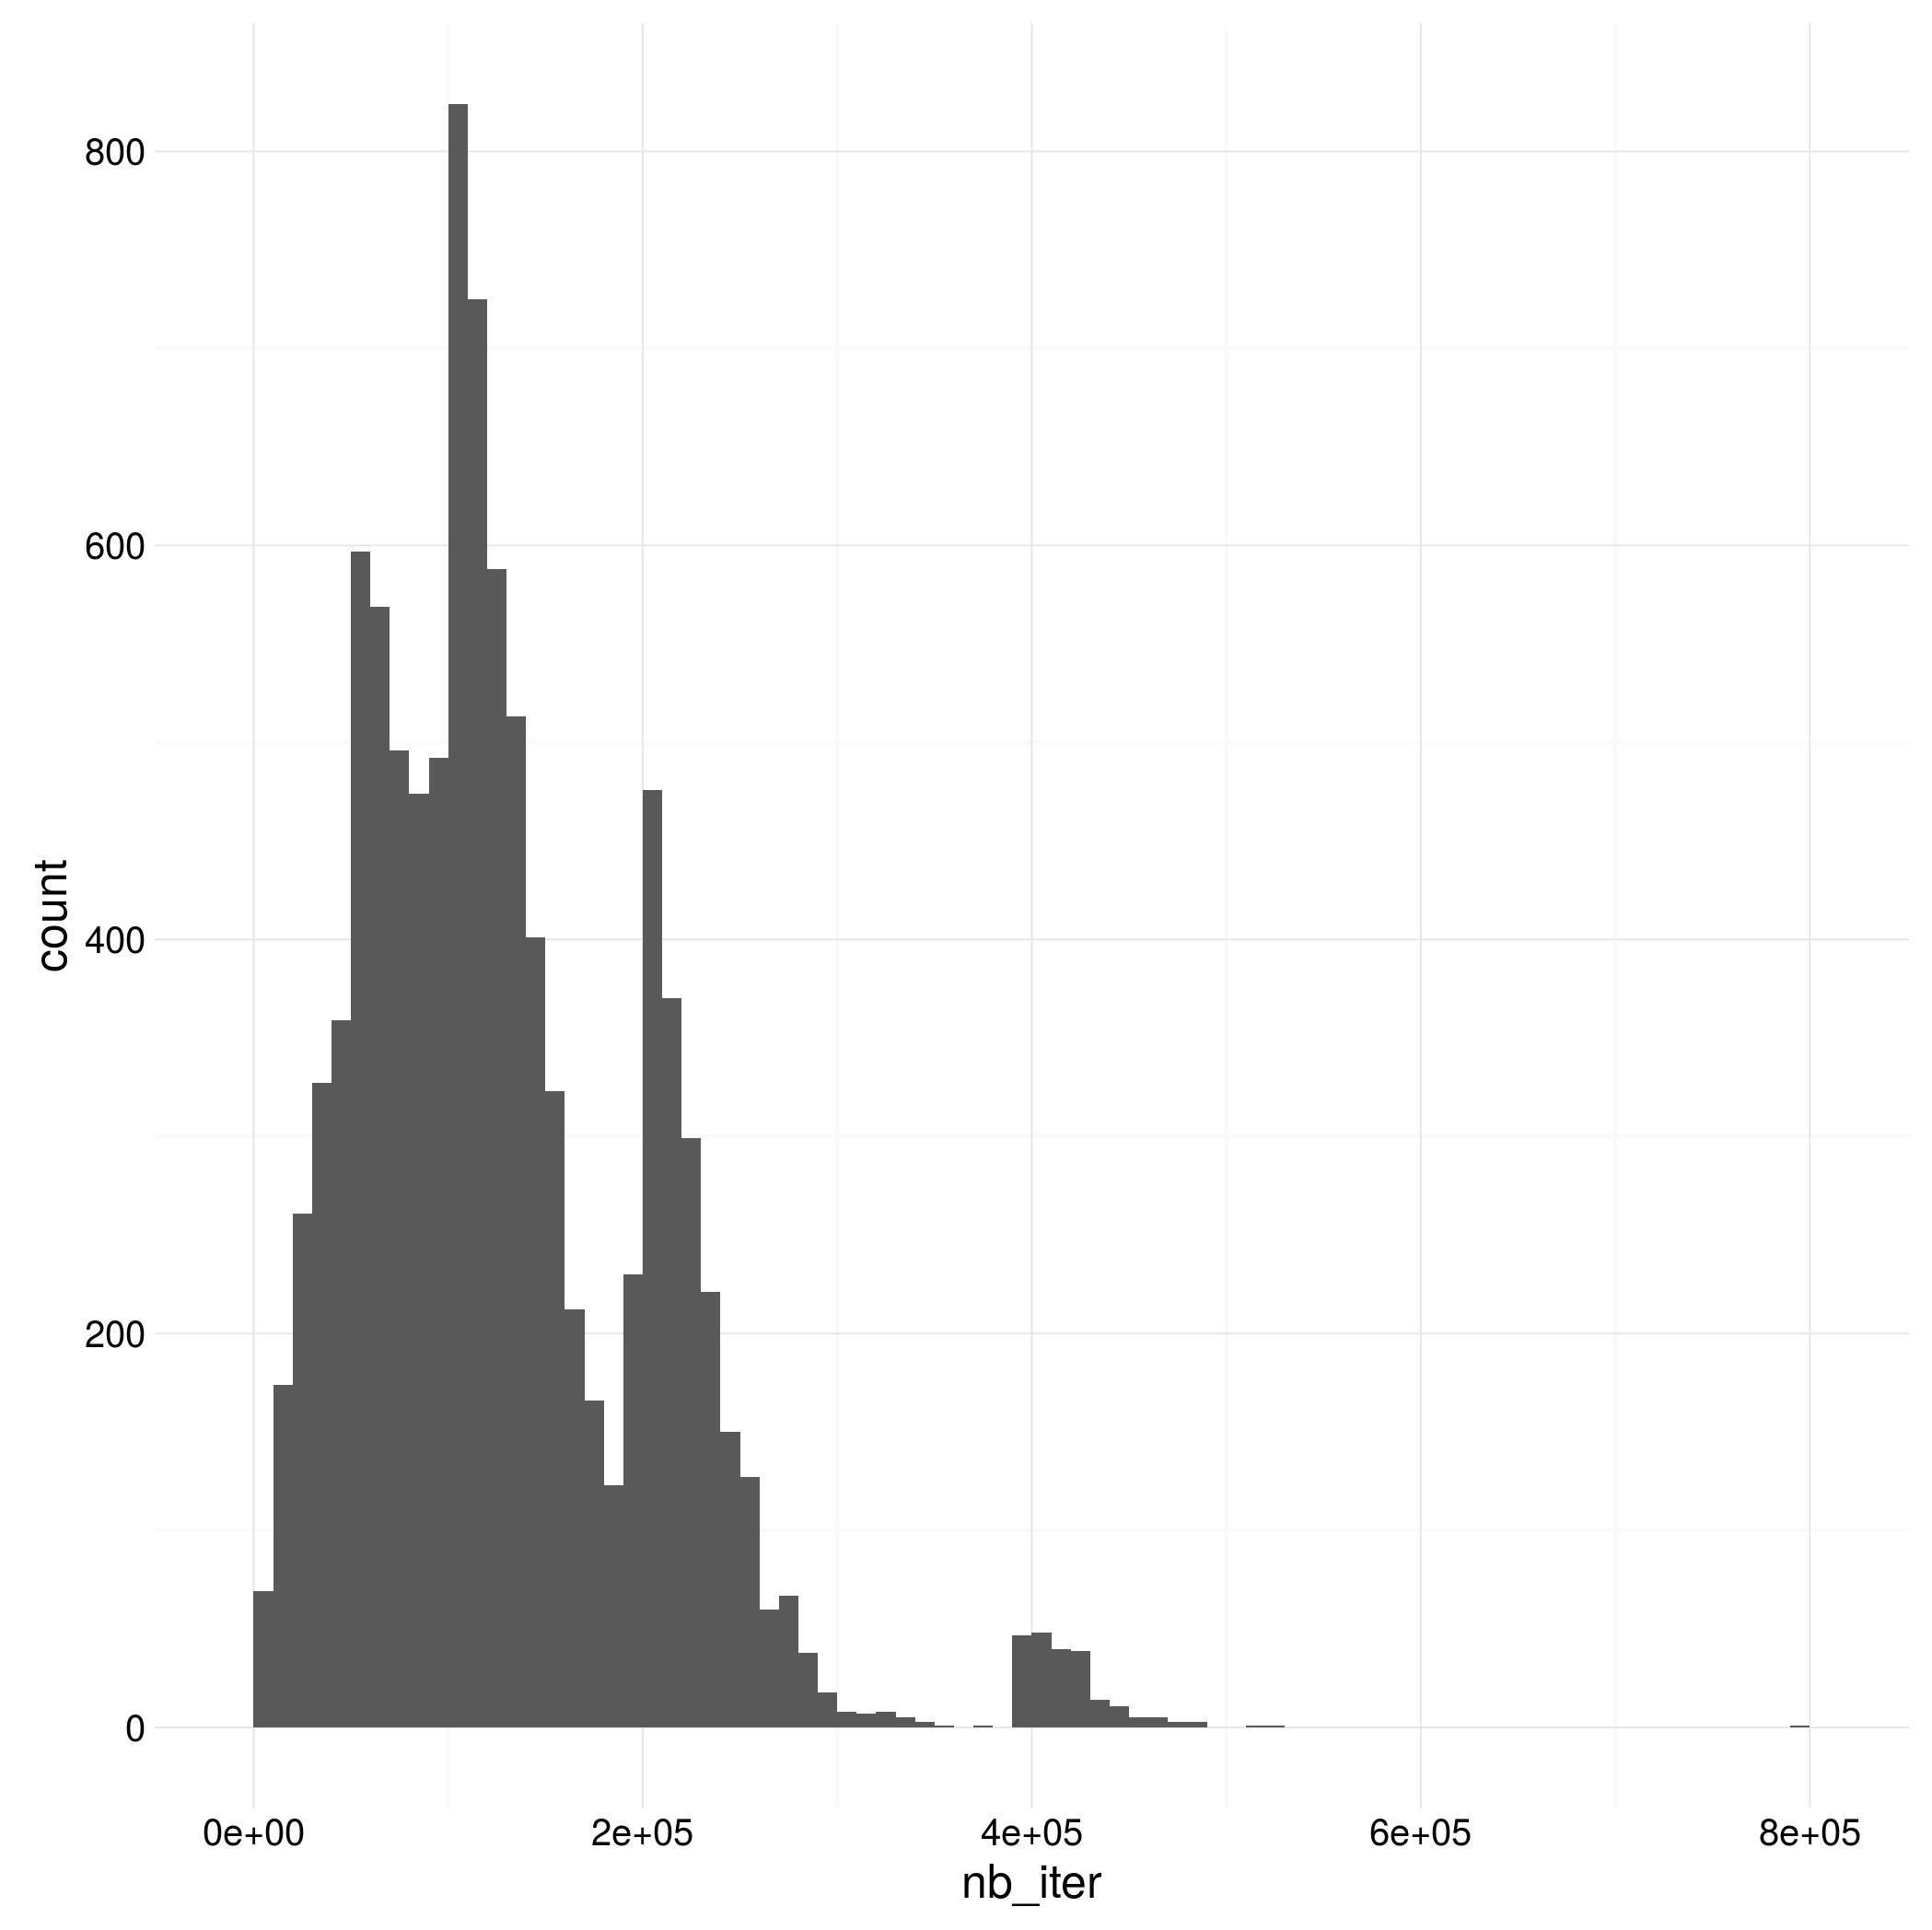
\includegraphics[keepaspectratio,scale=0.5]{./R/Images/Collisions.png}} \\
    \tiny{Histogramme du nombre d'appels de \texttt{brentrec} } \\
    \tiny{pour la recherche de collisions de la fonction} \\
    \tiny{\texttt{sip\_hash\_fix\_32} sur un ensemble de 10000 clés}
  \end{tabular}
\end{center}
Pour un algorithme utilisant une table de hashage et mémorisant les termes successifs de la suite nous nous attendions à obtenir une valeur moyenne du nombre d'exécution de siphash proche de la moitié de la taille de l'espace des hashs (voir Section résistance aux collisions). L'algorithme de Brent nécessite sans doute un peu plus d'évaluations de la fonction \texttt{siphash\_fix\_32} qu'un tel algorithme mais son fonctionnement "sans mémoire" rends possible la recherche de collisions sur des espaces de hash plus grands.
En effet, on mesure avec la commande \texttt{time} Le temps en seconde nécessaire pour le calcul de 10000 collisions:
\begin{lstlisting}[basicstyle={\scriptsize\ttfamily}, columns={fixed}, frame={}]
  33.48user 9.84system 0:55.27elapsed
\end{lstlisting}
Ce qui correspond à environ 3 ms pour le calcul d'une collision.
N'étant pas limité par la mémoire nous pourrions envisager de chercher, avec l'algorithme de Brent, des collisions pour la fonction \texttt{siphash}.
En effet on a, en moyenne, $2^{17}$ évaluations de \texttt{siphash\_fix\_32} permettent de detecter une collision en 3ms.
Pour \texttt{siphash} (version 64 bits), si on estime à $2^{33}$ le nombre d'évaluations nécessaires, alors il suffirait d'environ 196 secondes pour détecter une collision.
\subsection{Conditions expérimentales}
\subsubsection {Infos Cpu}
la commande \texttt{lscpu} permet d'afficher les informations liées aux processeurs.
\begin{lstlisting}[columns=fixed,basicstyle=\scriptsize\ttfamily]
Architecture :                           x86_64
Mode(s) opératoire(s) des processeurs :  32-bit, 64-bit
Boutisme :                               Little Endian
Processeur(s) :                          8
Liste de processeur(s) en ligne :        0-7
Thread(s) par cœur :                     2
Cœur(s) par socket :                     4
Socket(s) :                              1
Nœud(s) NUMA :                           1
Identifiant constructeur :               GenuineIntel
Famille de processeur :                  6
Modèle :                                 94
Nom de modèle :                          Intel(R) Core(TM) i7-6700 CPU @ 3.40GHz
Révision :                               3
Vitesse du processeur en MHz :           799.987
Vitesse maximale du processeur en MHz :  4000,0000
Vitesse minimale du processeur en MHz :  800,0000
BogoMIPS :                               6818.00
Virtualisation :                         VT-x
Cache L1d :                              32K
Cache L1i :                              32K
Cache L2 :                               256K
Cache L3 :                               8192K
Nœud NUMA 0 de processeur(s) :           0-7
Drapaux :                                fpu vme de pse tsc msr pae mce cx8 apic sep mtrr pge mca cmov pat pse36 clflush dts acpi mmx fxsr sse sse2 ss ht tm pbe syscall nx pdpe1gb rdtscp lm constant_tsc art arch_perfmon pebs bts rep_good nopl xtopology nonstop_tsc cpuid aperfmperf tsc_known_freq pni pclmulqdq dtes64 monitor ds_cpl vmx smx est tm2 ssse3 sdbg fma
cx16 xtpr pdcm pcid sse4_1 sse4_2 x2apic movbe popcnt tsc_deadline_timer aes xsave avx f16c rdrand lahf_lm abm 3dnowprefetch cpuid_fault intel_pt tpr_shadow vnmi flexpriority ept vpid fsgsbase tsc_adjust bmi1 hle avx2 smep bmi2 erms invpcid rtm mpx rdseed adx smap clflushopt xsaveopt xsavec xgetbv1 xsaves dtherm ida arat pln pts hwp hwp_notify hwp_act_window hwp_epp
\end{lstlisting}

\printbibliography
\end{document}
